
\documentclass[12pt,letterpaper,noanswers]{exam}
\usepackage[usenames,dvipsnames,svgnames,table]{xcolor}
\usepackage[margin=0.9in]{geometry}
\renewcommand{\familydefault}{\sfdefault}
\usepackage{tikz}
\usepackage{multicol}
\pagestyle{head}
\header{AM 111 Class 24}{}{Artificial Neural Networks, p.\thepage}
\runningheadrule
\headrule
\usepackage{siunitx}
\usepackage{graphicx} % more modern
\usepackage{amsmath} 
\usepackage{amssymb} 
\usepackage{hyperref}
\usepackage{tcolorbox}
\usepackage{enumitem}
\def\mbf{\mathbf}
\newcommand{\vc}[1]{\boldsymbol{#1}}
\def\dsst{\displaystyle}
\DeclareMathOperator*{\argmin}{arg\,min} % thin space, limits underneath in displays
\usepackage[numbered,autolinebreaks,useliterate]{mcode}

\begin{document}
 \pdfpageheight 11in 
  \pdfpagewidth 8.5in

\noindent 

\section*{Preliminaries}


\begin{itemize}
\itemsep0pt
\item Project update is due on Friday (accepted on Monday).
\item Presentation in class on Tuesday: 1 person team: 2 minutes. 2 person team: 3.5 minutes. 3 person team: 4.5 minutes.  Slides due (team submission) by 9am on Tuesday Nov 29.
\item Quiz 02 is on Thursday Dec 1 (topic info is on Canvas).
\item My office hours are in my office (Pierce 316) today.
\end{itemize}


\noindent\textbf{Big picture}

Today: modeling nonlinear functions using artificial neural networks

\vspace{0.2cm}
\hrule
\vspace{0.2cm}


\noindent \textbf{Teams}
\begin{multicols}{3}
1. Mina, Ivonne, Emma

2.  RJ, Johan, Shang

3. Benjamin, Julia K, Dani

4. Nini, Mack, Daniyal

5. Kevin G, Julia M, Nina

6. Jack, Caitlin, Esmé

7. Cameron, Robert, Tom

8. Ray, Alex H, Jessica

9. Eli, Basil, Zachary

10.  Kevin C, Eric, Brian

11. Eletria, Sophia, Aidan

12. Alex B, Nicolas, Marissa

\end{multicols}

\section*{Artificial neural networks}


\subsection*{Example: MNIST}

This example uses the MNIST (modified NIST) handwriting dataset \cite{lecun1998gradient}.

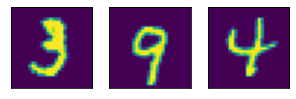
\includegraphics{img/C23mnist.png}

\begin{tcolorbox}
\begin{itemize}
\itemsep0pt
    \item The input is $28\times 28$ ($784$) pixels with values from $0$ to $255$.  The output is a digit, $0,1,...,9$.
\item To set up the model: the input layer has $784$ nodes.  Use one hidden layer with $300$ nodes.  For the output layer, use $10$ nodes, with each encoding one digit, $0$-$9$.  This will represent the digit $3$ by $0,0,0,1,0,0,0,0,0,0$
\item For the activation function, choose the logistic, $\sigma(x)$ for $\varphi_1$ and $\varphi_2$.
\item For the error function: use a sum of squares.  Let $y_0,...,y_9$ be the output of the nodes (corresponding to digits $0$ to $9$) and $\hat{y}_0^n$,...,$\hat{y}_9^n$ be the true values for a training data $n$. 

Let $\vc{e} = \vc{\hat{y}}^n-\vc{y}$, and $E_n(\vc{w}) = \vc{e}\cdot\vc{e} = \sum\limits_{i=0}^9 (\hat{y}_i^n-y_i)^2$
\end{itemize}
\end{tcolorbox}

\renewcommand{\inputnum}{1} 
\renewcommand{\hiddennum}{1}
\renewcommand{\outputnum}{1}
\begin{tikzpicture}
% Input Layer
\foreach \i in {1,...,\inputnum}
{
    \node[circle, 
        minimum size = 8mm,
        fill=orange!30] (Input-\i) at (0,-\i) {};
}
% Hidden Layer
\foreach \i in {1,...,\hiddennum}
{
    \node[circle, 
        minimum size = 8mm,
        fill=teal!50,
        yshift=0*5 mm
    ] (Hidden-\i) at (2.5,-\i) {};
}
% Output Layer
\foreach \i in {1,...,\outputnum}
{
    \node[circle, 
        minimum size = 8mm,
        fill=purple!50,
        yshift=(\outputnum-\inputnum)*5 mm
    ] (Output-\i) at (5,-\i) {};
}
% Connect neurons In-Hidden
\foreach \i in {1,...,\inputnum}
{
    \foreach \j in {1,...,\hiddennum}
    {
        \draw[->, shorten >=1pt] (Input-\i) -- (Hidden-\j);   
    }
}
% Connect neurons Hidden-Out
\foreach \i in {1,...,\hiddennum}
{
    \foreach \j in {1,...,\outputnum}
    {
        \draw[->, shorten >=1pt] (Hidden-\i) -- (Output-\j);
    }
}
\draw (Input-1) node {$784$};
\draw (Hidden-1) node {$300$};
\draw (Output-1) node {$10$};
\end{tikzpicture}
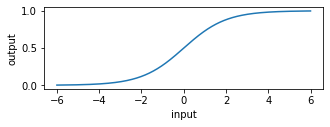
\includegraphics[scale=0.7]{img/C23logistic.png}

\begin{enumerate}[resume=classQ]
\item $\delta_j^2 = \dfrac{\partial E}{\partial a_j^2}$ where $E = \sum\limits_{i=0}^9 (\hat{y}_i^n-y_i)^2 = (\hat{y}_0^n - y_0)^2 + (\hat{y}_1^n - y_1)^2 + ... + (\hat{y}_9^n - y_9)^2$ and $y_i$ is the model output: $y_i = \varphi_2(a_i^2)$.
\begin{parts}
\item $\varphi_2(x) = \sigma(x)$ where $\sigma(x) = (1+e^{-x})^{-1}$.  Find $\dfrac{d\sigma}{dx}$, the derivative of the logistic with respect to $x$.
\vspace{1in}
\item Show that your expression can be rewritten as $\sigma'(x) = \sigma(x)(1-\sigma(x))$
\vspace{1cm}
\item Find $\delta_3^2 = \dfrac{\partial E}{\partial a_3^2} = \dfrac{\partial E}{\partial y_3}\dfrac{\partial y_3}{\partial a_3^2}$.
\vspace{1in}

\item Show that your expression for $\delta_3^2$ can be written as $-2e_{3}y_3(1-y_3)$, where $e_3 = \hat{y}_3^n-y_3$
\vspace{1cm}
\end{parts}

From this, we have $\dfrac{\partial E_n}{\partial w_{ji}^2} = \delta_j^2 z_i^{1} = -2e_{j}y_j(1-y_j)z_i^1$

\end{enumerate}
\begin{tcolorbox}
For this example, $\dfrac{\partial E_n}{\partial w_{ji}^2} = \delta_j^2 z_i^{1} = -2e_{j}y_j(1-y_j)z_i^1$.

What about
$\dfrac{\partial E_n}{\partial w_{ji}^1} = \delta_j^1 x_i = \sigma'(a_j^1)(W^{2T}\vc{\delta}^2)_j x_i$? 

We have $\sigma'(a_j^1) = \sigma(a_j^1)(1-\sigma(a_j^1)) = z_j^1(1-z_j^1)$ so 
$\dfrac{\partial E_n}{\partial w_{ji}^1} =  z_j^1(1-z_j^1)(W^{2T}\vc{\delta}^2)_j x_i$ where $(W^{2T}\vc{\delta}^2)_j = \sum\limits_m w_{mj}^2(-2e_my_m(1-y_m))$.

Let $e_j^1 = \sum\limits_m w_{mj}^2(e_my_m(1-y_m))$.  Then $\dfrac{\partial E_n}{\partial w_{ji}^1} =  -2e^1_jz_j^1(1-z_j^1)x_i$
\end{tcolorbox}
\subsection*{More MNIST}
The MNIST training and test files are on Canvas and in the \texttt{shared\_data} folder of FAS On Demand.
\begin{enumerate}[resume=classQ]
\item Using C23mnist.ipynb, you might try some of the following:
\begin{parts}
\item Look at the the effect of changing the learning rate.  It is \texttt{alpha} in the code.
\item Test the impact of decreasing the number of runs for training, or of increasing the number.  You might save your weights after every $5000$ updates, and plot your error or your percent correctly classified vs the number of updates used to create the weights.
\item Remove the hidden layer, add a second hidden layer, or adjust the number of units in the hidden layer.
\item Backpropagate the signal, rather than the error, for $[0,0,1,...0]$ (the number $2$) or for a different number to generate a $784$-element vector.  Convert that to an image, and plot it.  What do you see?

\end{parts}
\end{enumerate}

\section*{Review}
\subsection*{Topics from Class 11-22}
\begin{itemize}
\itemsep0pt
    \item numerical differentiation
    \begin{itemize}
    \itemsep0pt
        \item symbolic differentiation
        \item finite differences: forward, backward, central
        \item truncation error (order of a method), roundoff error
        \item challenge using data (vs a function)
        \item Richardson extrapolation
        \item vectorizing code
    \end{itemize}
    \item numerical integration (quadrature)
    \begin{itemize}
    \itemsep0pt
        \item approximate $f(x)$ via a polynomial interpolant and integrate the interpolant
        \item Newton-Cotes: equally spaced nodes (closed includes endpoints of interval, open does not)
        \item trapezoid rule (closed N-C), Simpson's rule (closed N-C), midpoint rule (open N-C)
        \item composite versions of these rules (multiple panels rather than just one)
        \item degree of precision
        \item error ($h^n$)
        \item Richardson extrapolation (Romberg integration)
        \item adaptive quadrature
        \item Gaussian quadrature (maximize degree of precision)
        \item Monte Carlo integration
    \end{itemize}
    \item ordinary differential equations (initial value problems)
    \begin{itemize}
    \itemsep0pt
        \item Euler's method, improved Euler, midpoint method, RK4, backward Euler
        \item local truncation error, global truncation error
        \item explicit methods, implicit methods
        \item instability, absolute stability, A-stable
    \end{itemize}
    \item discrete Fourier transform
    \begin{itemize}
    \itemsep0pt
        \item decompose a sound wave into frequencies
        \item discrete Fourier basis
        \item DFT, inverse DFT
        \item fast Fourier transform (FFT)
        \item aliasing, Nyquist frequency
        \item DFT for interpolation
    \end{itemize}
    \item artificial neural networks
    \begin{itemize}
    \itemsep0pt
        \item feedforward neural networks
        \item network structure encodes information about the model
        \item activation functions
    \end{itemize}
\end{itemize}



\bibliographystyle{plain}
\bibliography{AM111references}

\end{document}